\section{Protocolo CAN} \label{seccion:ProtocoloCAN}
\subsection{Consideraciones previas}
En es este trabajo de tesis se decidió continuar el desarrollo de la arquitectura con BUS-CAN ya que este es de interés para los proyectos desarrollados en INVAP. Cabe aclarar que el objetivo principal de esta tesis no es llevar a cabo una comparación exhaustiva de protocolos de comunicación tolerantes a fallas, sino elegir la más indicada y que se adapte a las necesidades de INVAP. Por tal motivo, se expone, en esta sección, las características importantes de CAN.

\subsection{Introducción}
El bus CAN (Controller Area Network) fue desarrollado por Bosh. Comenzó su desarrollo en 1983 y tuvo su primer release en 1986. Fue estandarizada por la Organización Internacional de Estandarización (ISO) bajo el nombre de  ISO 11898. El Bus CAN surgió como respuesta al rápido crecimiento de la elctrónica en la industria automotriz \citep{esdWEB}. Este protocolo se definió con el objetivo de proveer comunicación determinística de sistemas distribuídos, y que necesiten un alto grado de confiabilidad. CAN permite la conectividad vía bus serial. El bus está compuesto por  2 cables que pueden estar blindados o on \citep{esdWEB}.

Las características de CAN que la convierten en un tentadora opción para la aplicación en el sector espacial, son:
\begin{itemize}
  \item Bajo costo
  \item Operabilidad en ambientes eléctricos complicados
  \item capacidades de tiempo real.
  \item facilidad en el uso
\end{itemize}

La especificaciones de CAN, originalmente desarrollados por Bosch cubre solamente las capas físicas y de enlaces de datos del modelo de referencia de ISO/OSI. Luego de la estandarización ISO provee detalles adicionales de la capa física de CAN.

A diferencia de otros protocolos como USB o Ethernet, CAN no envía grandes bloques de datos de un punto a otro. CAN envía mensajes cortos como temperatura, o RPM ( Revoluciones por minutos), y son enviados como broadcast a todo el sistema \citep{texasCAN}.

El protocolo de comunicación CAN, en su estandar ISO 11898, explica como la información viaja entre los dispositivos conectados a una arquitectura siguiente el modelo de OSI. La arquitectura planteada por la ISO 11898 se puede observar en la FIGURA \citep{texasCAN}

\begin{figure}[h]
 \centering
 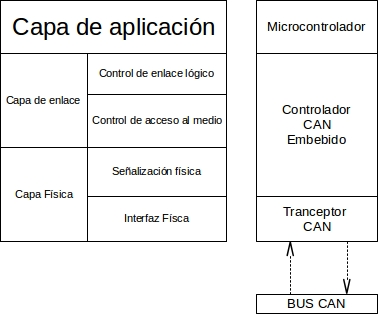
\includegraphics[scale=0.5]{images/Marco_teorico/ISO11898_Arquitectura_Standar.jpg}
  \caption{Arquitectura estándar propuesta por ISO898}
\label{fig:iso11898}
\end{figure}

En resumen, la capa física de CAN  describe la definición del bit timing, bit enconding y la sincronización, los niveles aceptables de la señal (corriente y voltaje), los conectores y características físicas de los cables \citep{texasCAN}. Por otro lado la capa de enlaces de datos, provee todos los servicios necesarios para la transmisión de un stream de bits desde un nodo a otro.

El bus CAN es un bus de tipo broadcast, es decir que todos los nodos escuchan todas las transmisiones. No hay manera de enviar un mensaje a un determinado nodo, por lo tanto no es necesario el direccionamiento de nodos. \citep{kvaserWEB}.

Actualmente la industria aeronáutica la utiliza. También el área agrícola en sus maquinarias, control de tráfico, sistemas de control industrial, sistemas domóticos y además, en equipamientos médicos.

\subsection{Elementos necesarios}
Como se puede observar en la Figura \ref{fig:iso11898}

Cada nodo conectado a la red necesita de
\begin{itemize}
\item \ac{CPU}, o microprocesador, que decida que mensajes debe recibir y que debe enviar
\item Controlador CAN, muchas veces integrado en el controlador, el cual recibe la serie de bits del bus. También es el encargado de transmitir mensajes (cuando se requiera), esto significa que al mensaje lo convierte en una serie de bits.
  \item Tranceiver, definido en el ISO 11898.
\end{itemize}


% \subsection{Capa física}
\subsection{Capa física}\label{subsec:capafisca}
El estándar de CAN define el bit enconding, el timing, y la sincronización. La capa física es la encargada de convertir 1 y 0 en pulsos eléctricos para enviar mensajes por el canal, y también el proceso inverso cuando recibe mensajes. La capa física es implementada enteramente en \ac{HW} \citep{texasFISICACAN}.

\subsubsection{Bus de comunicación}
Para iniciar una transmisión de mensaje es necesario como mínimo dos nodos conectados al bus CAN. Esto se debe a que el dispositivo que envía un mensaje está también recibiendo su propio mensajes, con esto puede chequear cada bit que ha enviado. De esta manera, un segundo nodo responde con un ACK, mientras el bit todavía está siendo transmitido por el primer nodo. Esto demuestra por qué se necesitan de dos nodos para completar la transmisión de mensajes \citep{texasFISICACAN}.

En la Figura \ref{fig:traficBUSCAN} se observa un ejemplo extraído de \citep{texasFISICACAN}. En esta se muestra un nodo A que envía un mensaje. Luego se ve que que B y C contestan con un ACK indicando que el mensaje fue recibido sin errores. Luego B y C comienzan a transmitir hasta que C gana el bus debido a que tiene un bit dominante, y termina este completando su mensaje.

\begin{figure}[h]
 \centering
 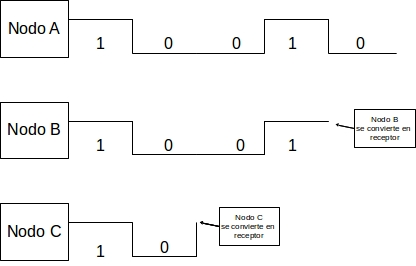
\includegraphics[scale=0.3]{images/Marco_teorico/CAN_BUS_Traffic.jpg}
  \caption{Tráfico en el BUS CAN}
\label{fig:traficBUSCAN}
\end{figure}

El medio físico  es una línea de bus con dos cable, terminada por una resistencia. Los cables pueden ser paralelos, trenzados y/o blindandos. Los segmentos de cable para la conexión de los nodos deben ser lo más cortos posibles.

Para mayores detalle técnico referentes al bus será necesario estudiar el estándar ISO 11898 o en \cite{texasFISICACAN}.

El largo del bus va a determinar el bitrate de la comunicación. Para alcanzar un bitrate de 1Mbps, el máximo del canal de comunicación es de 40m. Si se tiene un bus de 1km el bitrate es de 0.05Mbps. Con esto se puede observar que el bitrate decae cuando la distancia se incrementa. Para CAN, el bitrate también está determinado por el total del delay del sistema \citep{texasFISICACAN}. Esto es la suma de los delays del nodo, y el delay propio del cable.

Debe destacarse que que existen diferentes capas físicas para el protocolo CAN:
\begin{itemize}
\item El tipo más común es el establecido en el estanar ISO 11898-2. Este protocolo cuenta con dos cables, cada uno identificado como CAN\_H y CAN\_L. También es llamado \textit{CAN de alta velocidad} (1 Mbit/s). Este requiere que el largo del cable sea como máximo 40m.
\item También en el estándar de ISO se establece el ISO 11898-3, el cual define otro esquema de doble cable balanceado pero para bajas velocidades. Este es tolerante a fallas si alguno de los cables entra en corto circuito. También es llamado también como \textit{CAN de baja velocidad} (125 kbit/s)
\item Se define el SAE J2411 que utiliza un solo cable para la capa física. Este es utilizado en autos (velocidad por encima de los 50 kbit/s). No tiene demasiados requerimientos en cuanto al bitrate ni el largo del canal de comunicación. El estandar define 32 nodos por red.
\item Existen modificaciones del estandar RS485 para su funcionamiento con CAN
\end{itemize}

\subsubsection{Bit timing}
El tipo de señal es codificado con Non Return Zero (NRZ). Los bits son codificados en dos estados llamados ``recesivo'' y ``dominante''(el bit 0 es asociado al bit dominante). El protocolo pemite acceso al bus multi-master con una resolución determinística ante colisiones. Para lograr la sincronización, el protocolo sincroniza durante las transiciones. Por tal motivo, deben evitarse el envío de largas cadenas de bits en un mismo estado. CAN utiliza una técnica que se denomina ``bit stuffing'' o ``bit padding'' en la cual luego de enviar 5 bits con el mismo estado, se insertan bits de relleno.

\subsubsection{Asignación eficiente del bus}
La asignación del bus depende de su aplicación. Generalmente existen 2 tipos de clases de asignación.

\begin{itemize}
\item \textbf{Asignación en un tiempo fijo}: La asignación se hace secuencialmente a cada participante sin importar si este necesita el bus en ese momento. Esta técnica, asigna tiempo del bus a cada nodo, y si no tiene nada que enviar, el bus se encuentra ocioso.

\item \textbf{Asignación en base a sus necesidades}: el bus se asigna según las necesidades del nodo (utilizando CSMA o CSMA/CD). En CAN la asignación del bus es negociado entre los mensajes que esperan ser transmitido. CAN utiliza esta técnica.
\end{itemize}


% \subsection{Capa de enlace}
\subsection{Capa de Enlace}
CAN utiliza el control de acceso al medio tipo \textit{CSMA/CS+CR} (Acceso múltiple con detección de portadora, detección de colisión más resolución de colisión). CAN resuelve el problema de la colisión con la supervivencia de una de las tramas que chocan en el bus. La trama ``ganadora'' es aquella que tiene mayor prioridad. Por lo tanto se puede indicar que CAN por naturaleza tiene en cuenta la prioridad.

Como ya se mencionó anteriormente el bit \textit{dominante} es el 0 y el bit \textit{recesivo} es el 1, la resolución se realiza con una operación lógica AND de todos los bits transmitidos simultaneamente. Cada transmisor se encuentra continuamente
observando y comprobando que el bit recibido se corresponda con el bit que envía. Cuando no coincide, el controlador retira el mensaje del bus y se convierte automáticamente en receptor. Como puede observarse la capa de enlace se comparta de manera similar a la capa física.

La única diferencia que presenta la capa de enlace de CAN es que todos los errores a nivel de un solo bits son detectados. Los errores de múltiples bits son detectados con una alta probabilidad \citep{can-ciaWEB}.


% \subsection{Formato del mensaje}
\subsection{Formato del mensaje}
CAN utiliza un formato de mensajes cortos (94 bits) En el mensaje no está explícito ninguna dirección, por este motivo el mensaje puede ser escuchado por todos los nodos de la red \citep{kvaserWEB}.

Los tipos de mensajes son los siguientes:
\begin{itemize}
    \item Frame de datos (Data Frame)
    \item Frame remoto (Remote Framte)
    \item Frame de error (Error Frame)
    \item Frame de sobrecarga (Overload Frame)
\end{itemize}

\subsubsection{Data Frame}
Este es el frame más común. Las partes más importantes son:

\begin{itemize}
\item Campo de arbitraje, el cual determina la prioridad del mensaje
\item El campo de datos, que contiene desde cero hasta ocho bytes de datos
\item El CRC, que está conformado por 15 bits utilizados para calcualr el checksum del mensaje
\item Un campo de ACK. Cualquier controlador que haya recibido el mensaje envía un bit de acuse de recibo al final de cada mensaje. El transmisor comprueba la presencia del bit ACK. En caso de no detectar este bit reenvía el mensaje. Al no poder conocer la dirección de los nodos, no se sabe si el mensaje fue recibido correctamente por el node receptor, solo se sabe que el mensaje fue recibido por uno o más nodos.   
\end{itemize}

\subsubsection{Remote Frame}
El frame remoto es un Data Frame con dos diferencias, es marcado como Remote Frame, esto es el bit RTR es recesivo; y por otro lado no hay un campo de datos. Este frame es utilizado para pedir la transmisión de un determinado frame de datos. Por ejemplo si el nodo A transmite un Remote Frame con el campo de arbitraje en 234, entonces el nodo B, reponderá con un frame de datos con el campo de arbitraje seteado a 234 \citep{kvaserWEB}. Este frame es poco utilizado.

\subsubsection{Error Frame}
Este frame se envía cuando un node detecta alguna falla en el mensaje. El envío de este frame provoca la retransmisión inmediata del mensaje. El Error Frame consiste en una bandera, el cual está compuesto por 6 bits del mismo valor, y un Error Delimiter que está compuesto por 8 bits recesivos.

\subsubsection{Overload Frame}
Este frame es similar al frame de error con el mismo formato. Es enviado cuando el nodo está ocupado. Este Frame es muy poco usado. El único controlador que generaba Overload Frame está obsoleto \citep{kvaserWEB}


\subsubsection{CAN estándar y CAN extendido}


